
\documentclass{article}

\usepackage{graphicx}
\usepackage{amsmath}

\usepackage[margin=1in]{geometry}


\def\hwtitle{Computational Physics HW3}
\def\hwauthor{Ethan Rooney}
\def\hwdate{2020-02-12}

\usepackage{fancyhdr}
\lhead{\hwauthor}
\chead{\hwtitle}
\rhead{\hwdate}
\lfoot{\hwauthor}
\cfoot{}
\rfoot{\thepage}
\renewcommand{\footrulewidth}{0.4pt}
\pagestyle{fancy}

\author{\hwauthor}
\title{\hwtitle}
\date{\hwdate}

\begin{document}

\maketitle
\thispagestyle{fancy}

\section{Introduction}
 
This weeks homework centers around the implementation of the Rutta-Kunga 2 method for numeric integrators.

I will be implementing this algorithm on a variety of systems, initially I will be modeling an idealized version of Earths orbit, assuming that the planet is in a perfectly circular orbit and then experimenting with more and more elliptical orbits to see show how the RK2 method begins to break when the linearity of a system varies drastically over a fixed time step. As seen in the highly eccentric orbit covered in problem 4. 

The core of the RK2 method is to find a better way to approximate an integral when compared to Euler's method. For RK2 once the differential equation is known, the slope at the initial time $t_0$ and initial position $x_0$ is computed, a half step is taken along that line, the approximate value of the slope at the midpoint is then calculated, and then a full step is taken along the newly computed slope of the equation from $(t_0, x_0)$ to $(t_i, x_i)$. For well behaved differential equations, this method provides a more accurate method of integration than Euler's method.

\begin{equation}
	k_1 = f(y'(t_0),t_0)
\end{equation}

\begin{equation}
	y_1(t_0 + \frac{h}{2}) = y'(t_0) + k_1\frac{h}{2}
\end{equation}

\begin{equation}
	k_2 = f(y_1(t_0+\frac{h}{2}), t_0 +\frac{h}{2})
\end{equation}

\begin{equation}\label{eq:rk2}
	y'(t_0+h) = y'(t_0)+k_2h 
\end{equation}

\section{Results}

\bigskip
\noindent{\bf Question 1}
\medskip


Given Equation \ref{eq:1}: if we let 
$ r = 1 \text{AU} $ 
and 
$ \ddot{r} = a_c $
we can then use Equation \ref{eq:2} to find 
$ GM_{\odot} = v^2r $.
We know that 
$ v $
is the tangential velocity of the earth, which must travel
$ 1 \text{AU} \times 2\pi \text{ rad} $
per 
$ 1 \text{ Year} $
we find 
$ GM_{\cdot} = 4\pi^2 \text{AU}^3\text{Year}^{-2} $.


\begin{equation}\label{eq:1}
	\ddot{r} = \frac{GM_{\odot}}{r^2}\hat{r}
\end{equation}
\begin{equation}\label{eq:2}
	a_c = \frac{v^2}{r}
\end{equation}


\bigskip
\noindent{\bf Question 2}
\medskip

Below in Figure \ref{fig:qual} we see the orbit of Earth as we would expect for the initial conditions given.

\begin{figure}[h]
	\begin{center}
		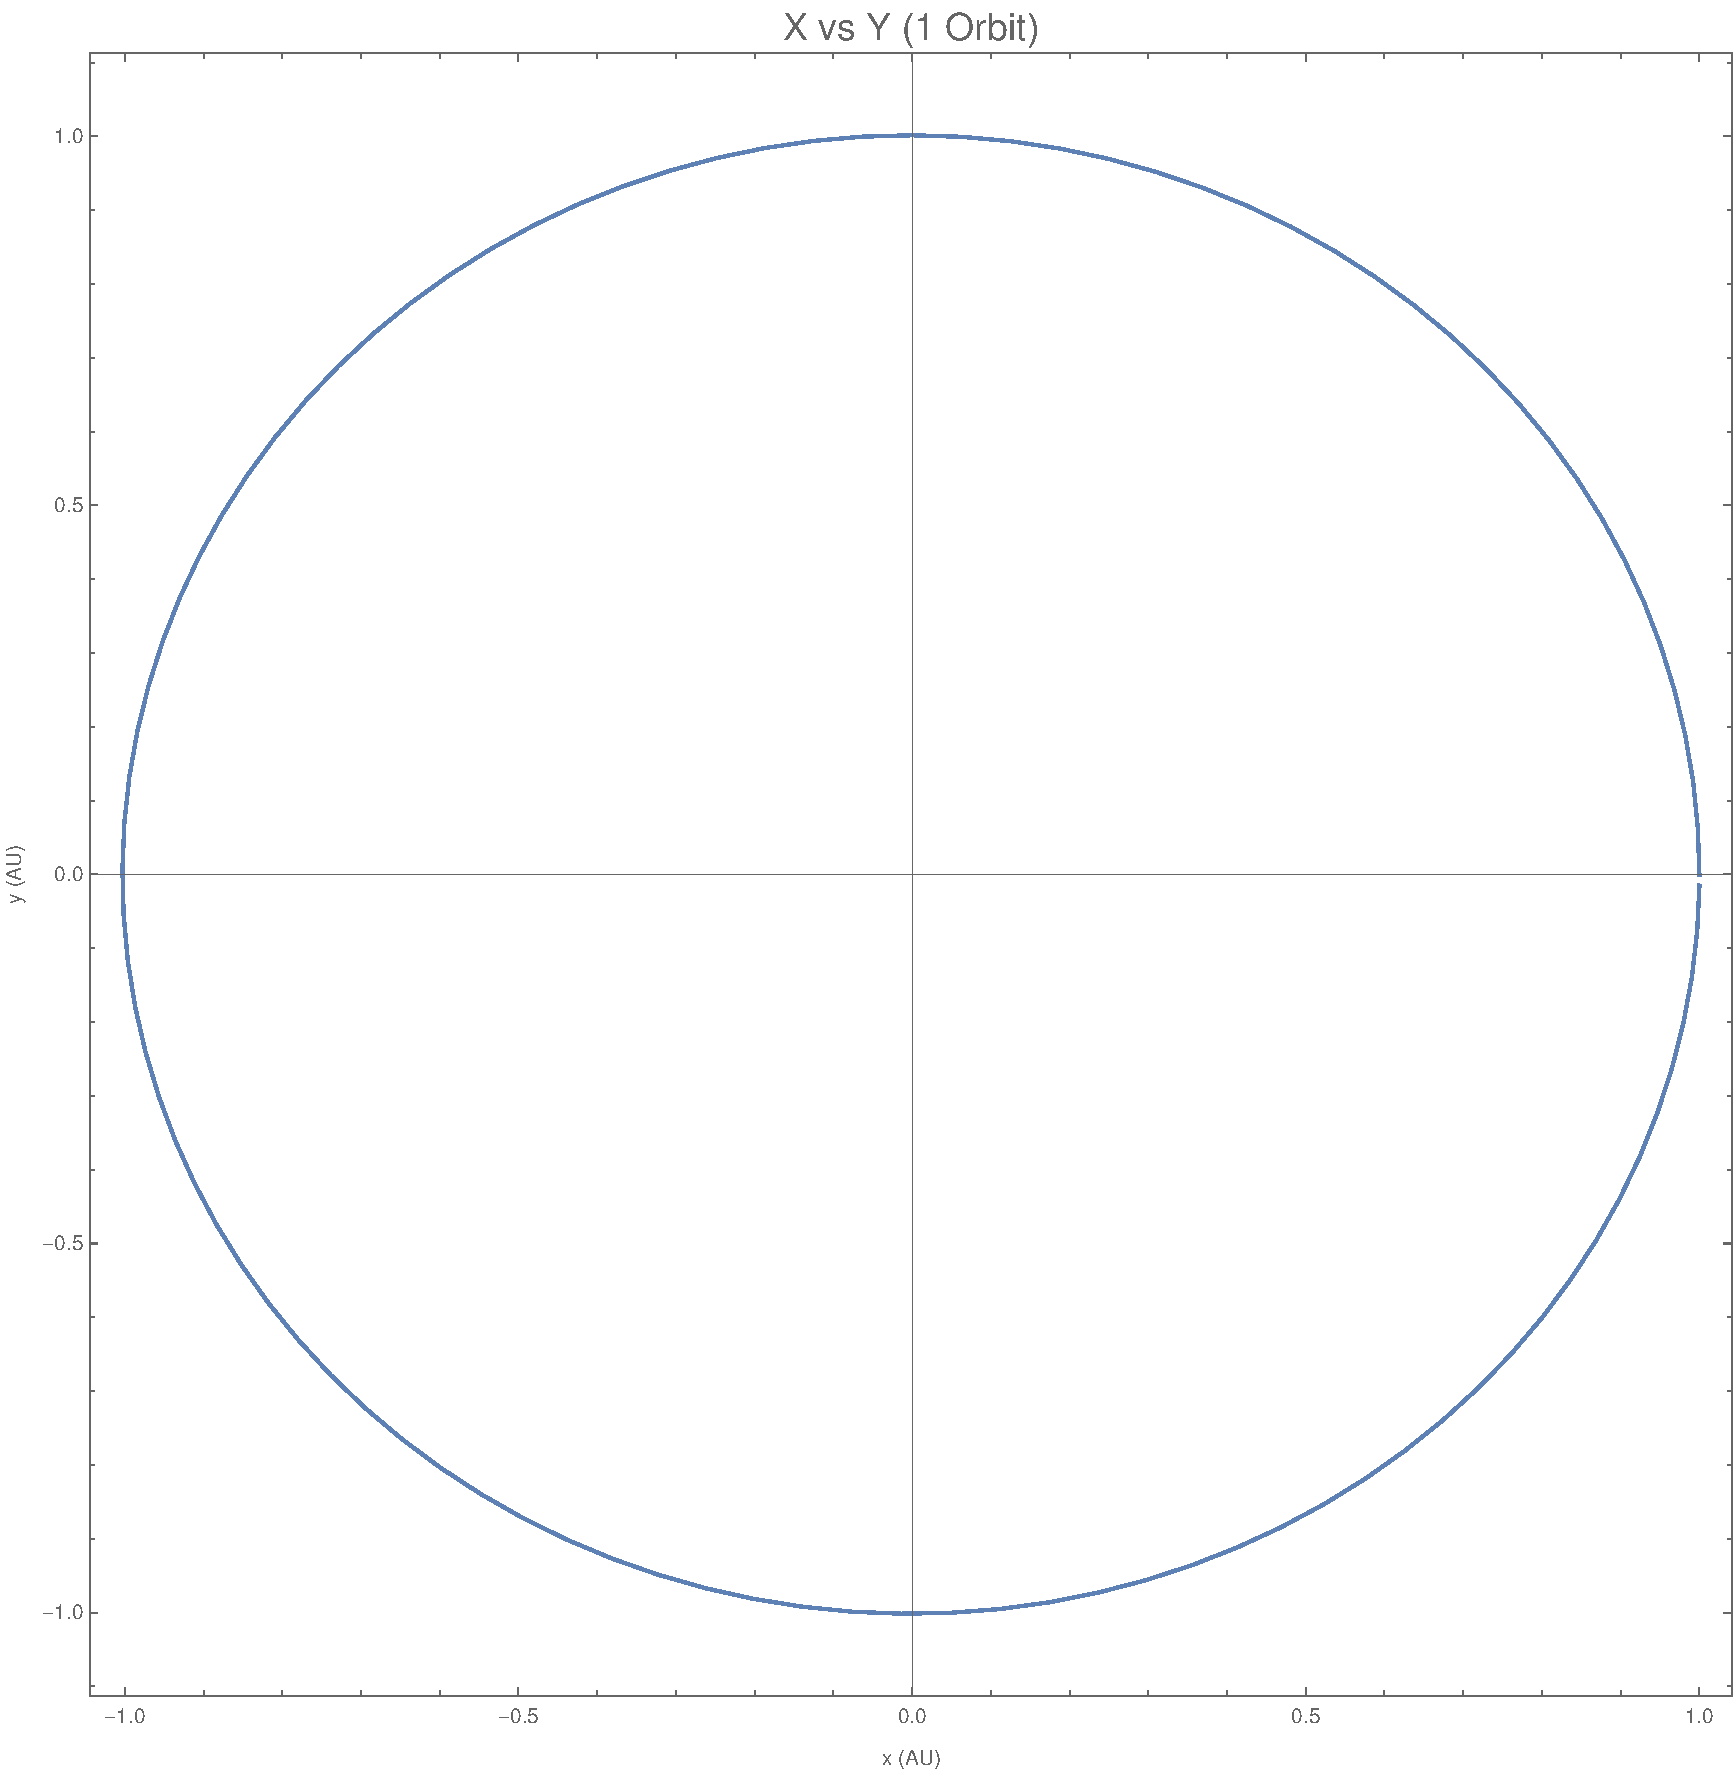
\includegraphics[width=0.4\textwidth]{qual.pdf}
	\end{center}
	\caption{Plot of the orbit of Earth as simulated with RK2}
\label{fig:qual}
\end{figure}

While in Figure \ref{fig:qual} we see how error in the conservation of energy scales with step size. The slope of the Log-Log plot is 3 (See Equation \ref{eq:3}).
This means that for a 10 fold increase in step size, the error of the integrator is reduced by 1000. This is consistent with the expected scaling of RK2.

\begin{figure}[h]
	\begin{center}
		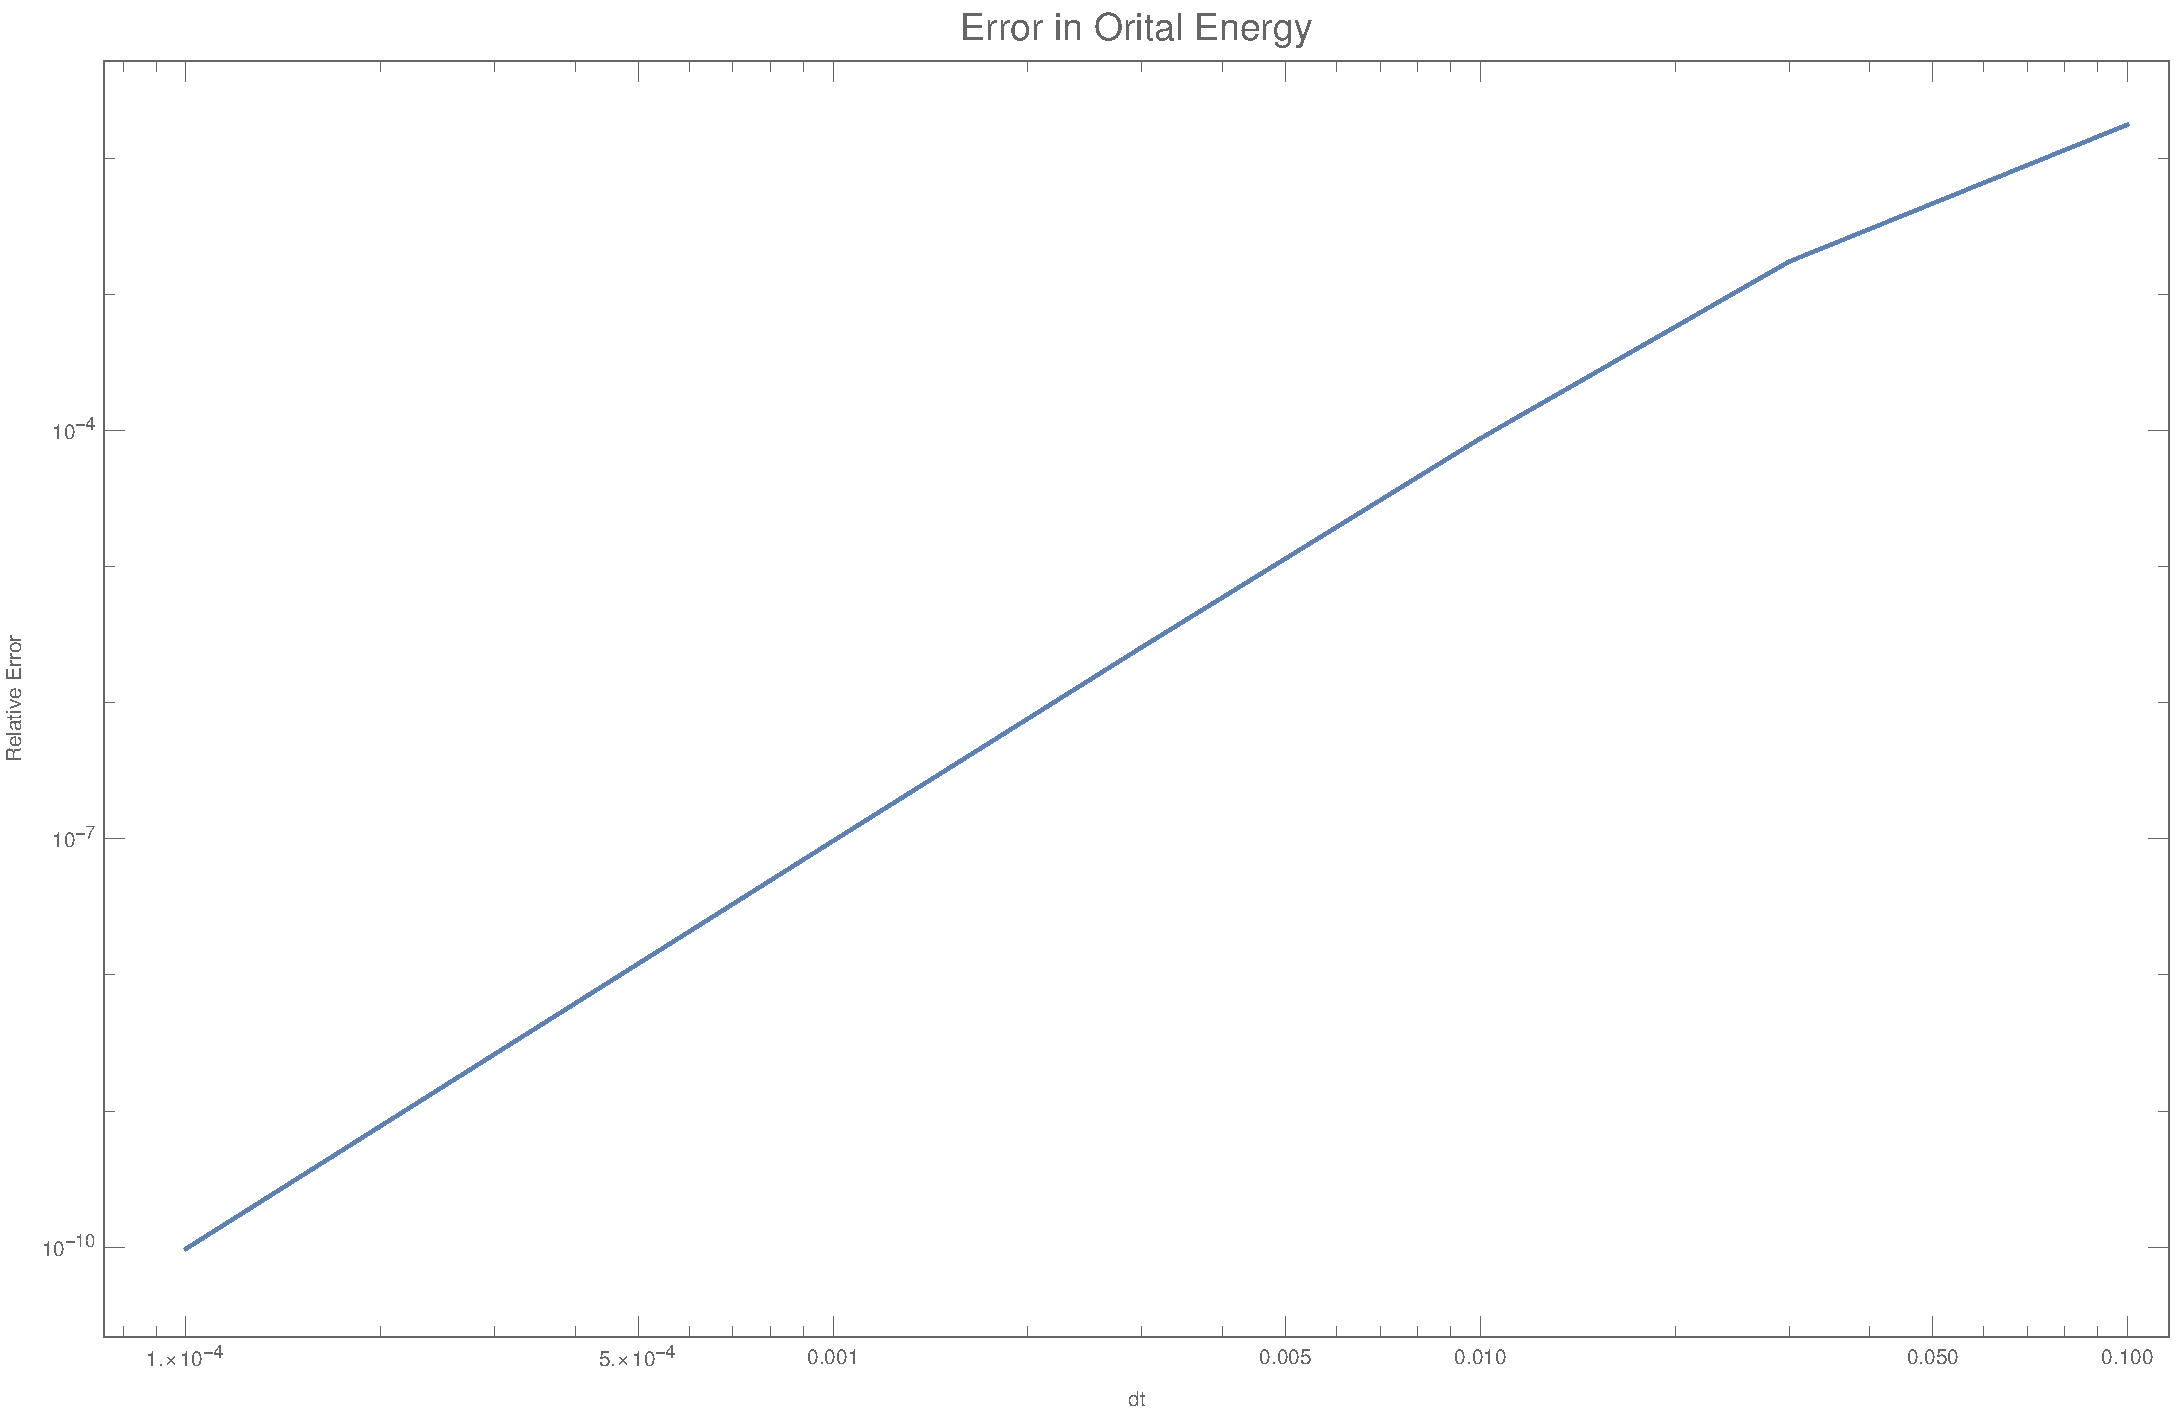
\includegraphics[width=0.4\textwidth]{error.pdf}
	\end{center}
	\caption{Error in the Energy Simulated by RK2 compared to Energy Conservation}
\label{fig:error}
\end{figure}

\begin{equation}\label{eq:3}
	Slope = \frac{log(y_1)-log(y_2)}{log(x_1)-log(x_2)}=\frac{log(0.01)-log(0.001)}{log(8.73084*10^{-5})-log(9.65174*10^{-8})} \simeq 3
\end{equation}

Based on the Above graph, the time step required for an accuracy of 1:1000 is $dt \simeq 0.0245$.

\pagebreak
\bigskip
\noindent{\bf Question 3}
\medskip

Seen in Figure \ref{fig:eccen} is an orbiting body with a Ratio of aphelion:perihelion of 1.857.

\begin{figure}[h]
	\begin{center}
		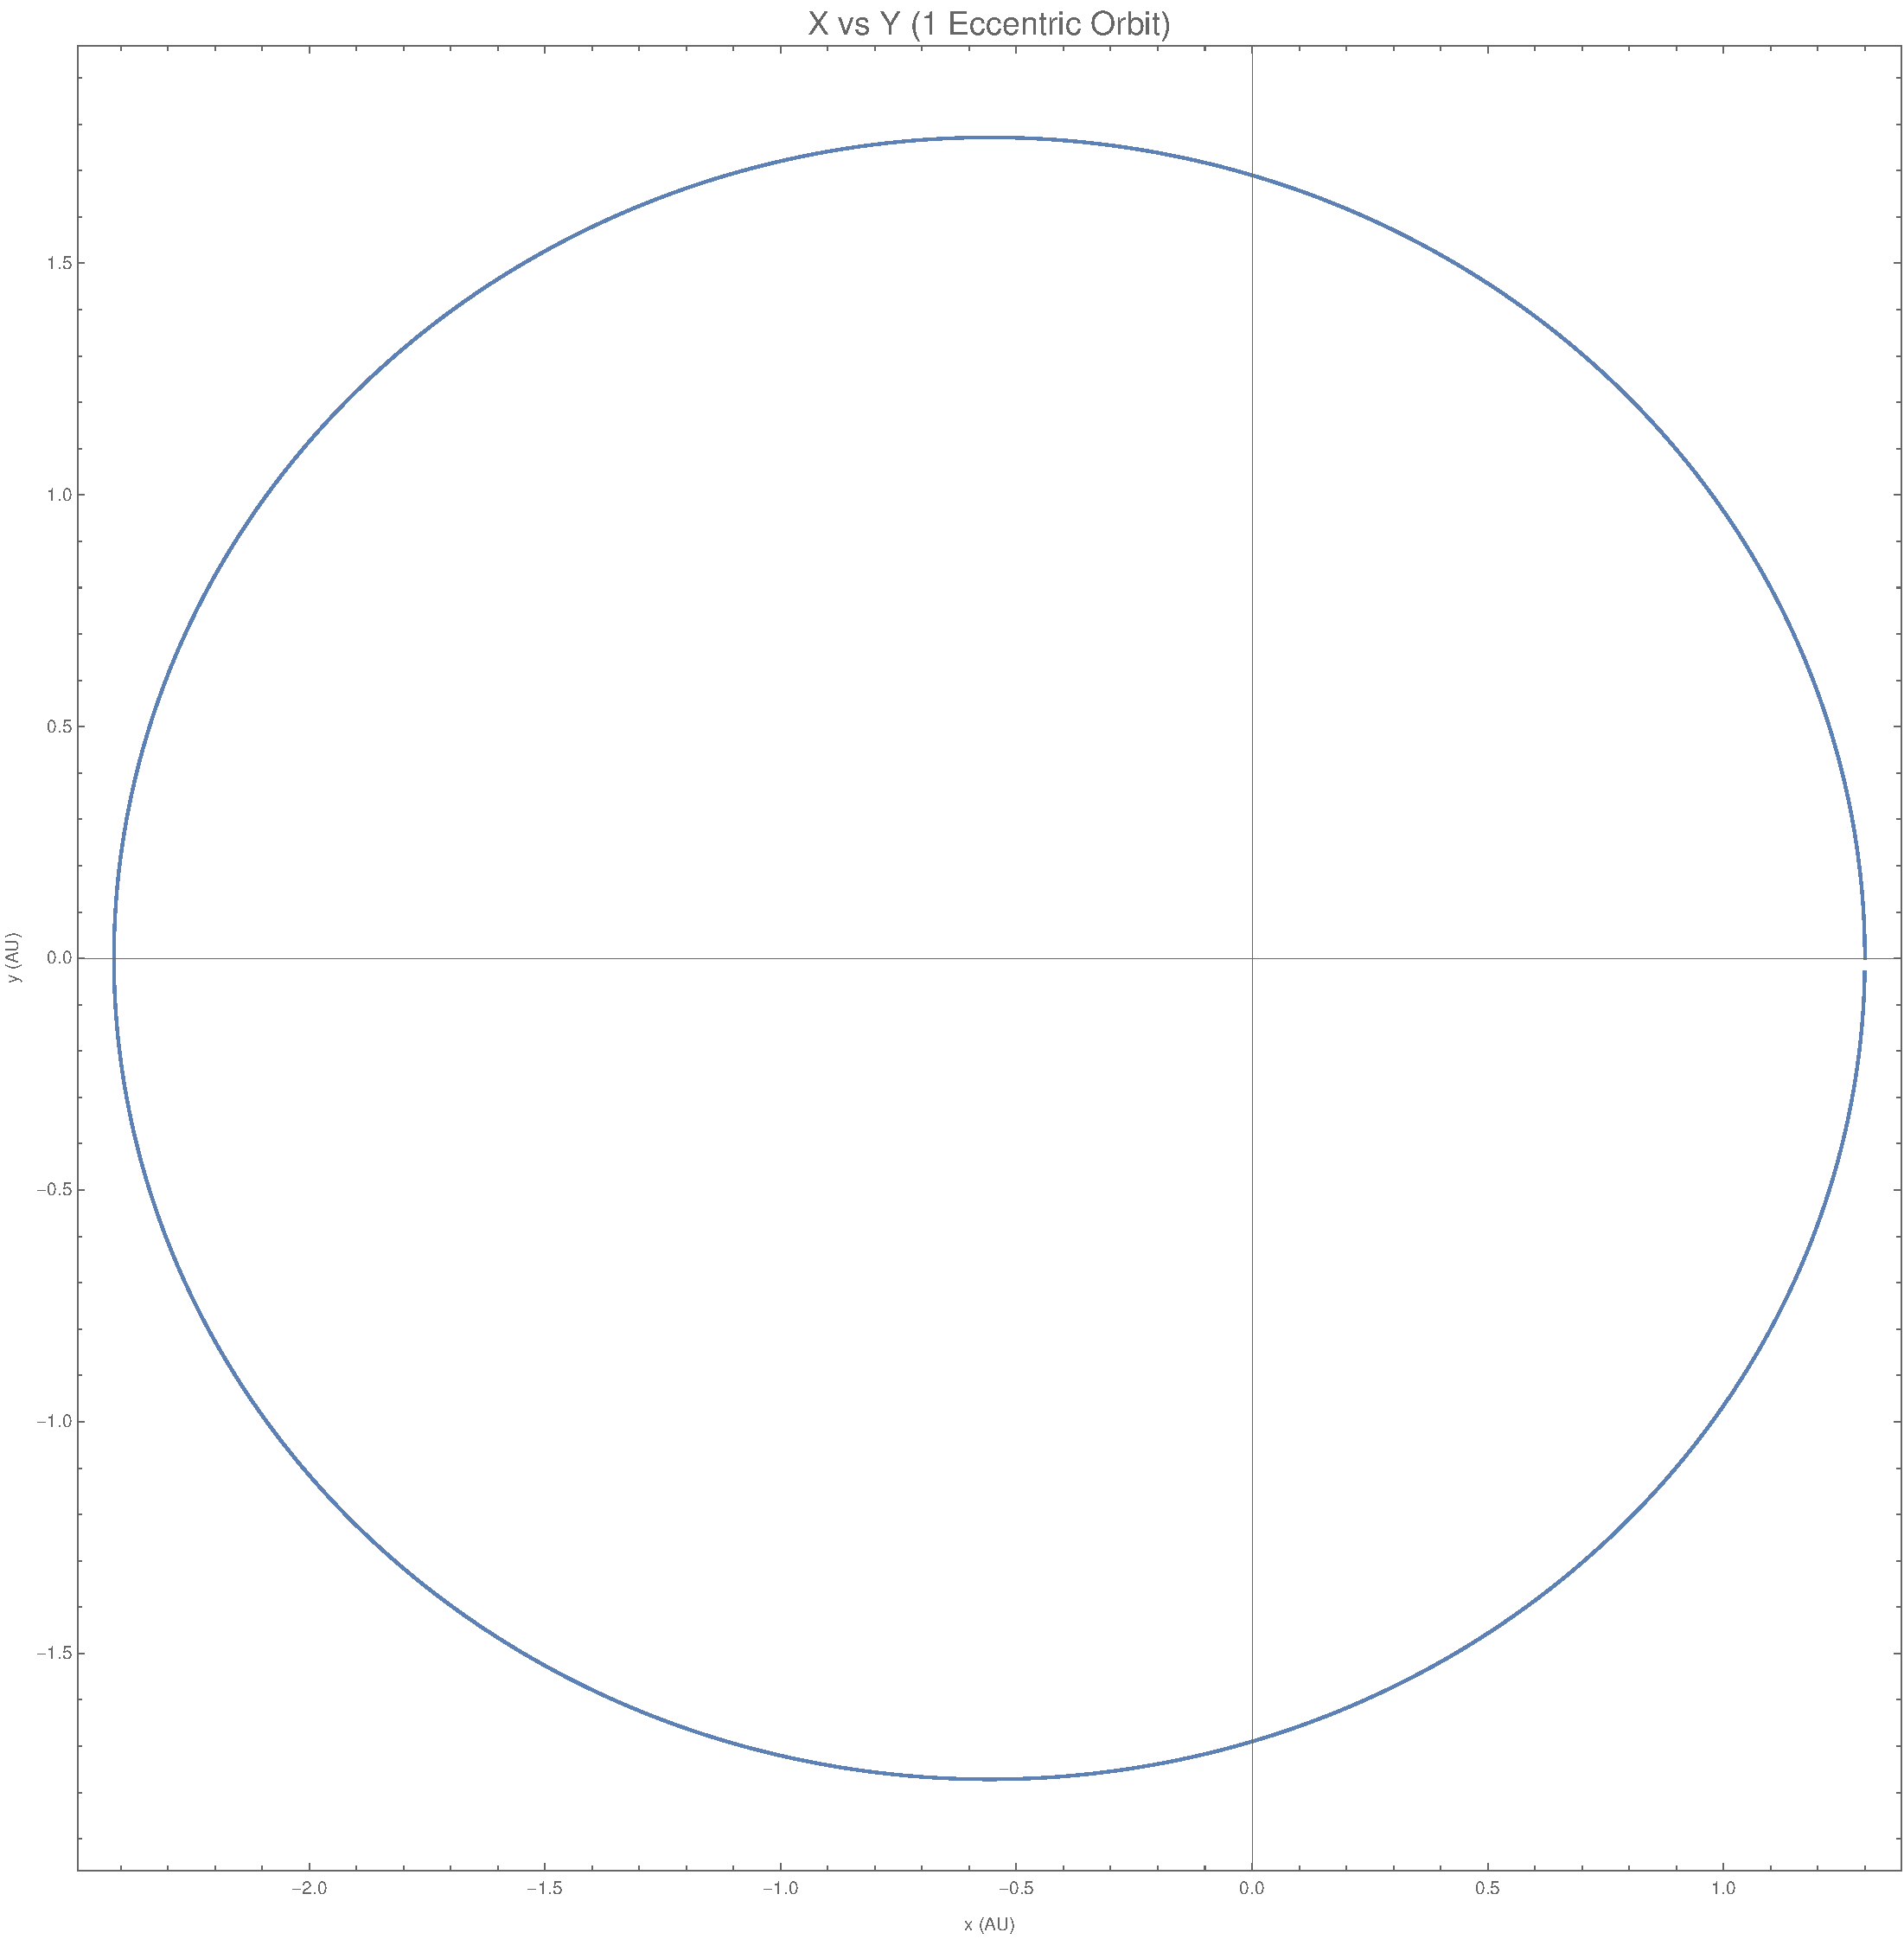
\includegraphics[width=0.4\textwidth]{eccen.pdf}
	\end{center}
	\caption{Eccentric Orbit of a Planet with Perihelion of 1.3 AU, with an initial velocity of $2\pi$ AU/Year.}
	\label{fig:eccen}
\end{figure}

In Figure \ref{fig:energy} We see the energy of the planet as it makes one complete Revolution. The Kinetic energy of the Planet is at a max when the Potential Energy is at a minimum, which occurs at Perihelion. Furthermore the Total energy of the system is constant and negative, indicative of a bound system. This is consistent with my expectations.

\begin{figure}[h]
	\begin{center}
		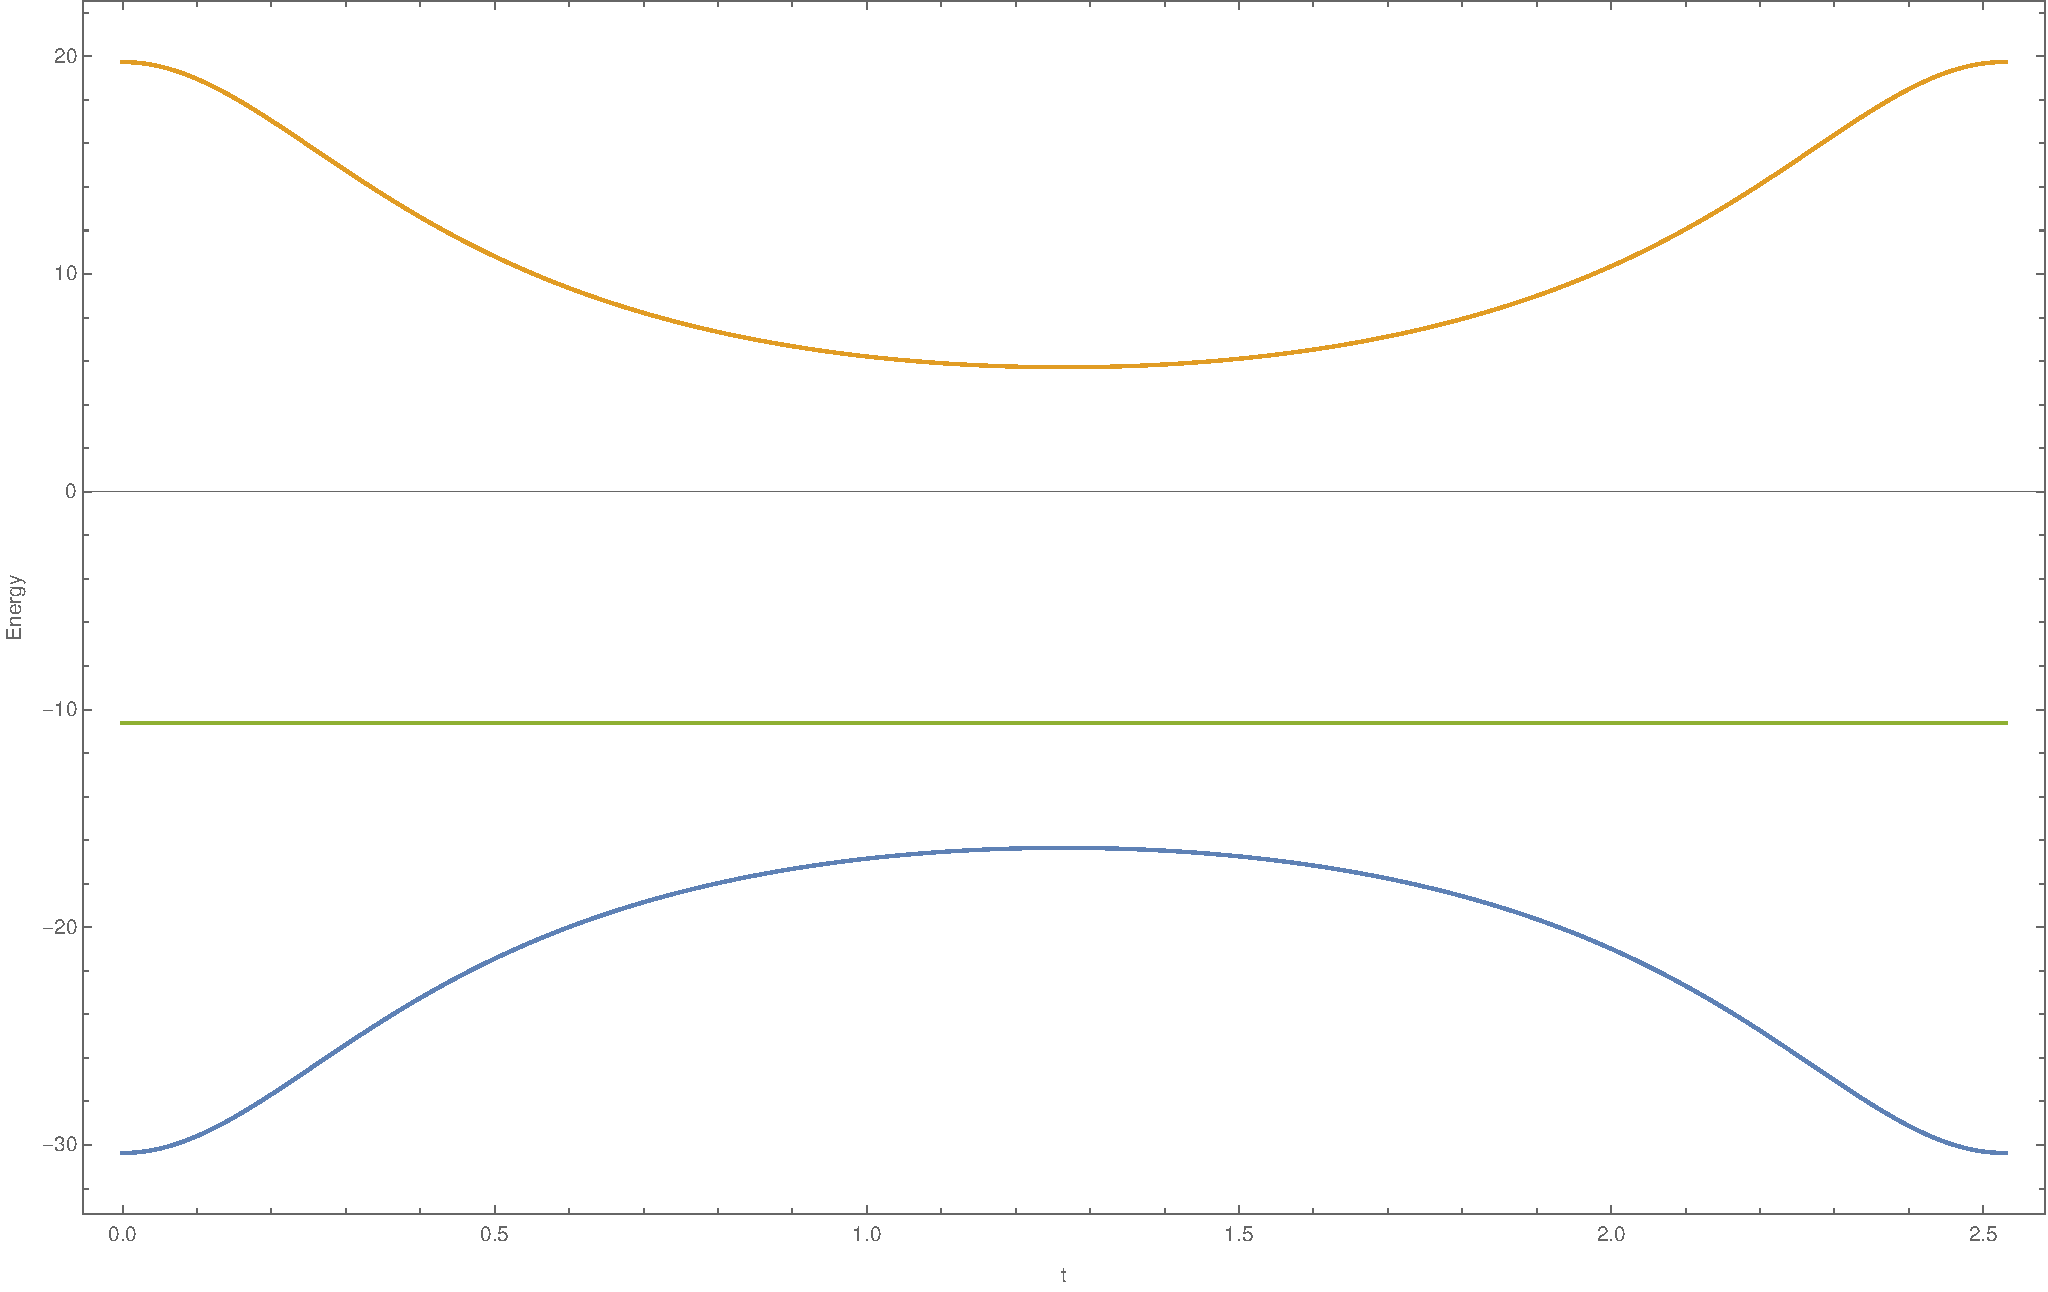
\includegraphics[width=0.4\textwidth]{energy.pdf}
	\end{center}
	\caption{The Energy of a slightly eccentric orbiting body. The orange line is the Kinetic Energy, the blue is Potential Energy, while Green is the total energy.}
\label{fig:energy}
\end{figure}


\pagebreak
\bigskip
\noindent{\bf Question 4}
\medskip

\begin{figure}[h]
	\begin{center}
		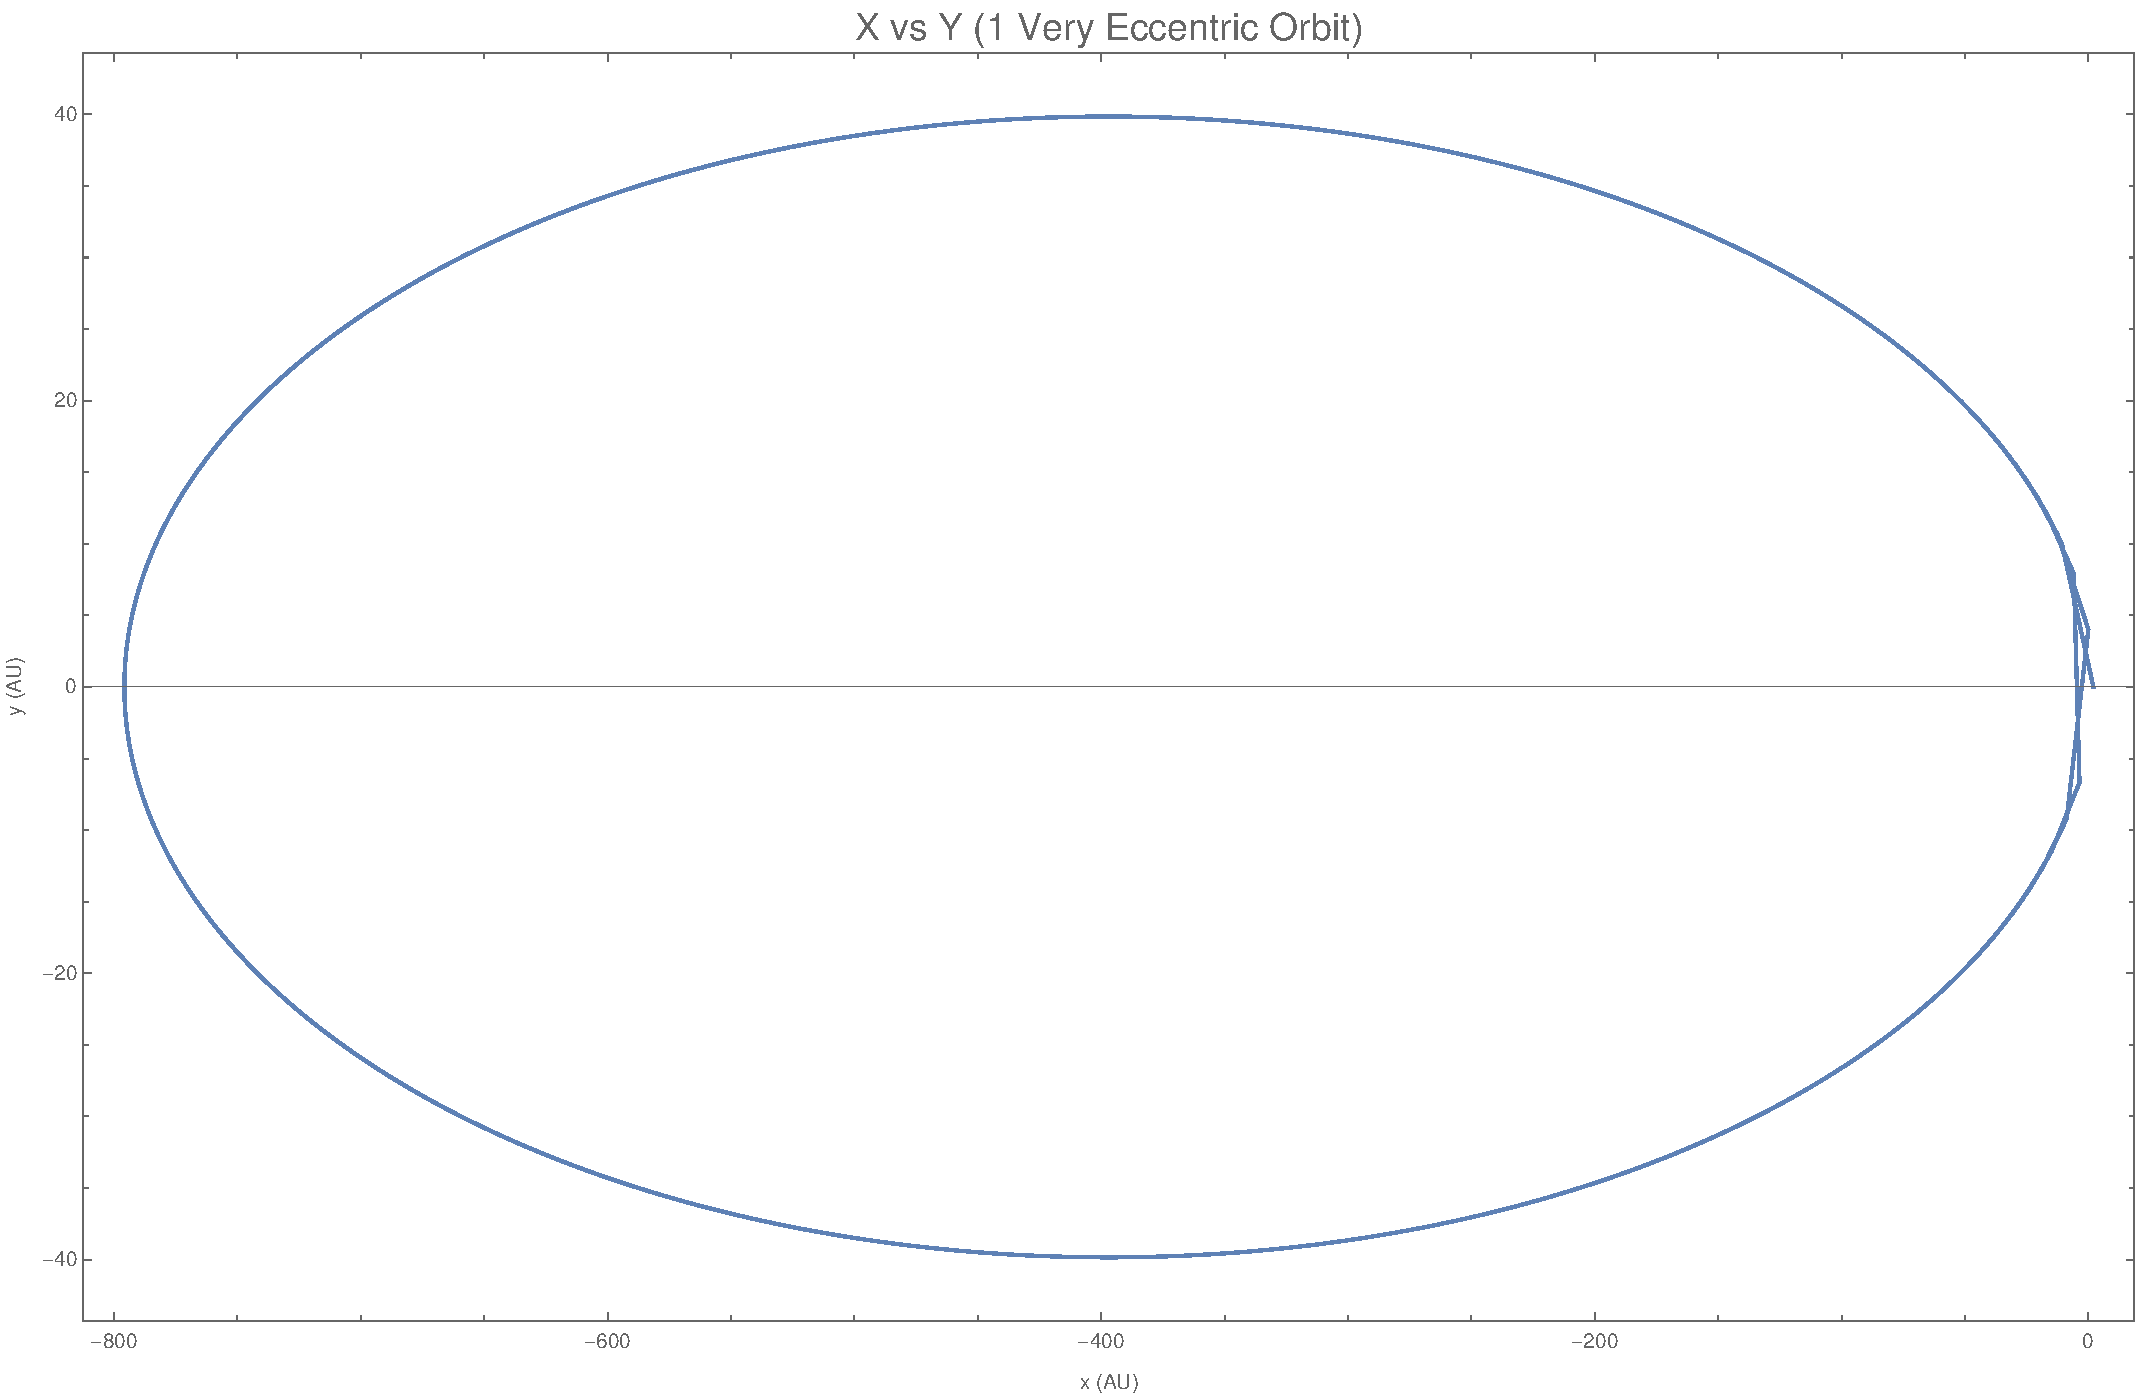
\includegraphics[width=0.4\textwidth]{veo3.pdf}
	\end{center}
	\caption{Orbit of an eccentric body over 20000 years with a time step of 0.001. Orbit is $\sim7970$ years long.}
	\label{fig:vee}
\end{figure}


\begin{figure}[h]
	\begin{center}
		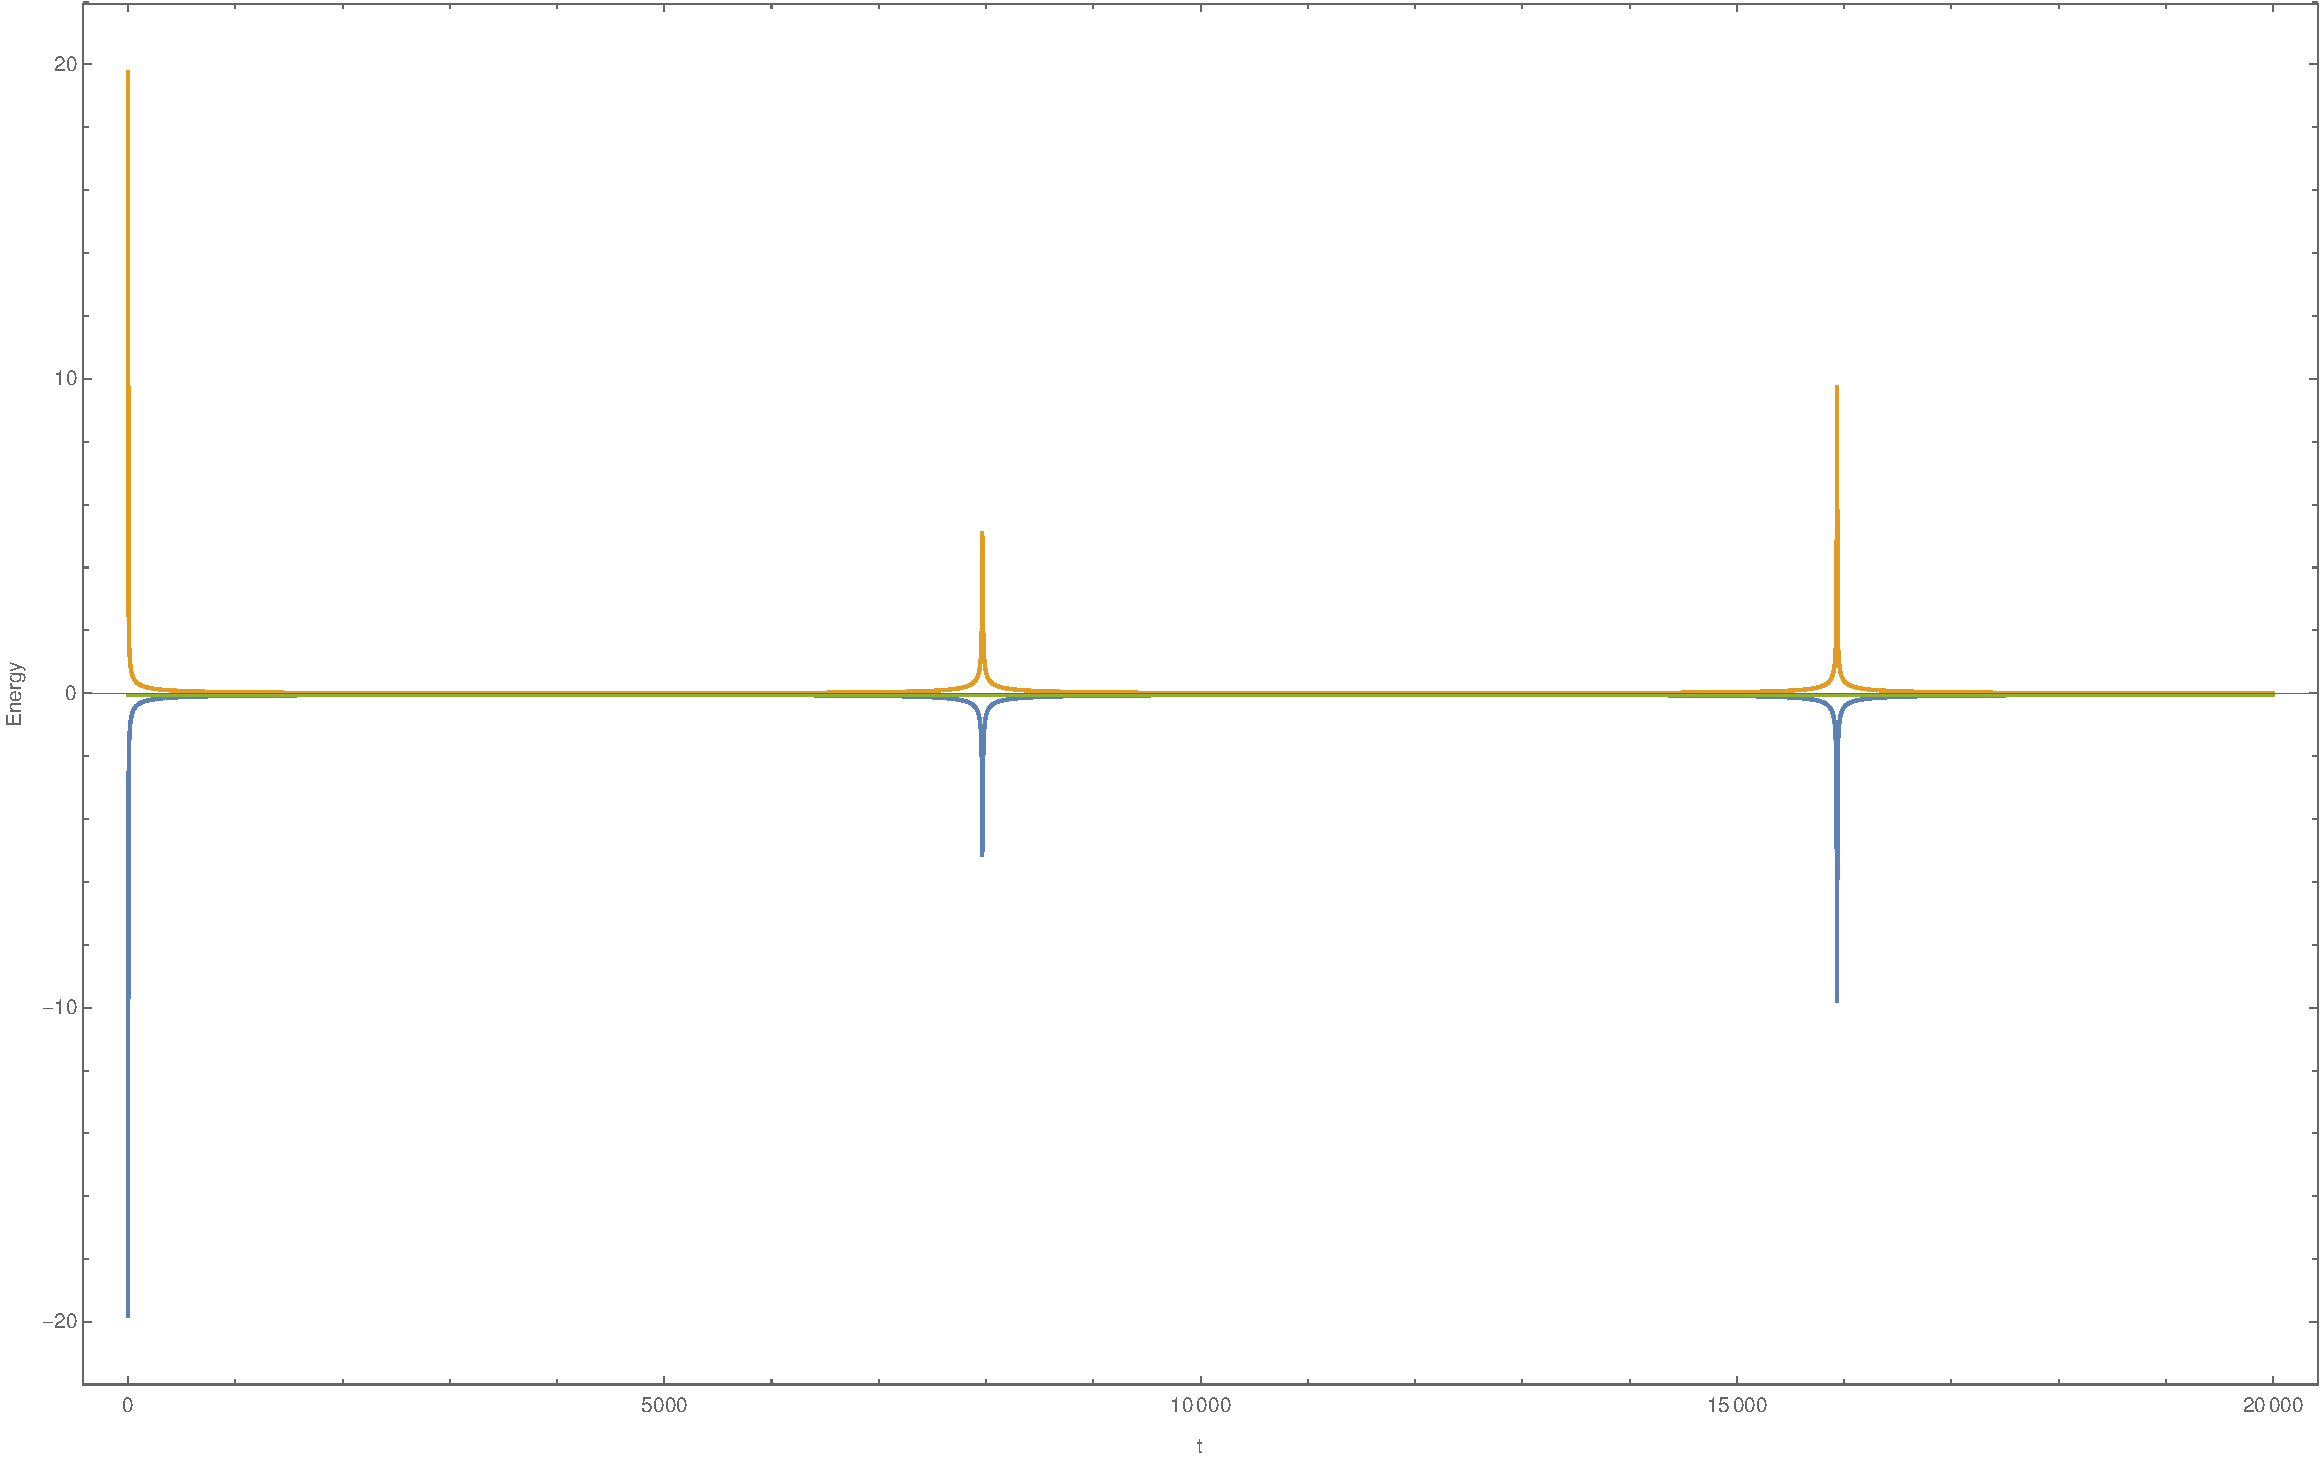
\includegraphics[width=0.4\textwidth]{veccenergy.pdf}
	\end{center}
	\caption{The Energy of a very eccentric orbiting body. Orange represents the Kinetic Energy, Blue the Potential Energy and Green the Total Energy}
	\label{fig:vee}
\end{figure}

In Figure \ref{fig:vee} see a plot of the energy transformation for a highly elliptical orbit with a period of $ ~7970 $ years the orbit behaves much the way I expect it to. The small artifacts near the perigee are due to the 5 year time steps used for plotting.

\pagebreak
\bigskip
\noindent{\bf Question 5}
\medskip

\begin{figure}[h]
	\begin{center}
		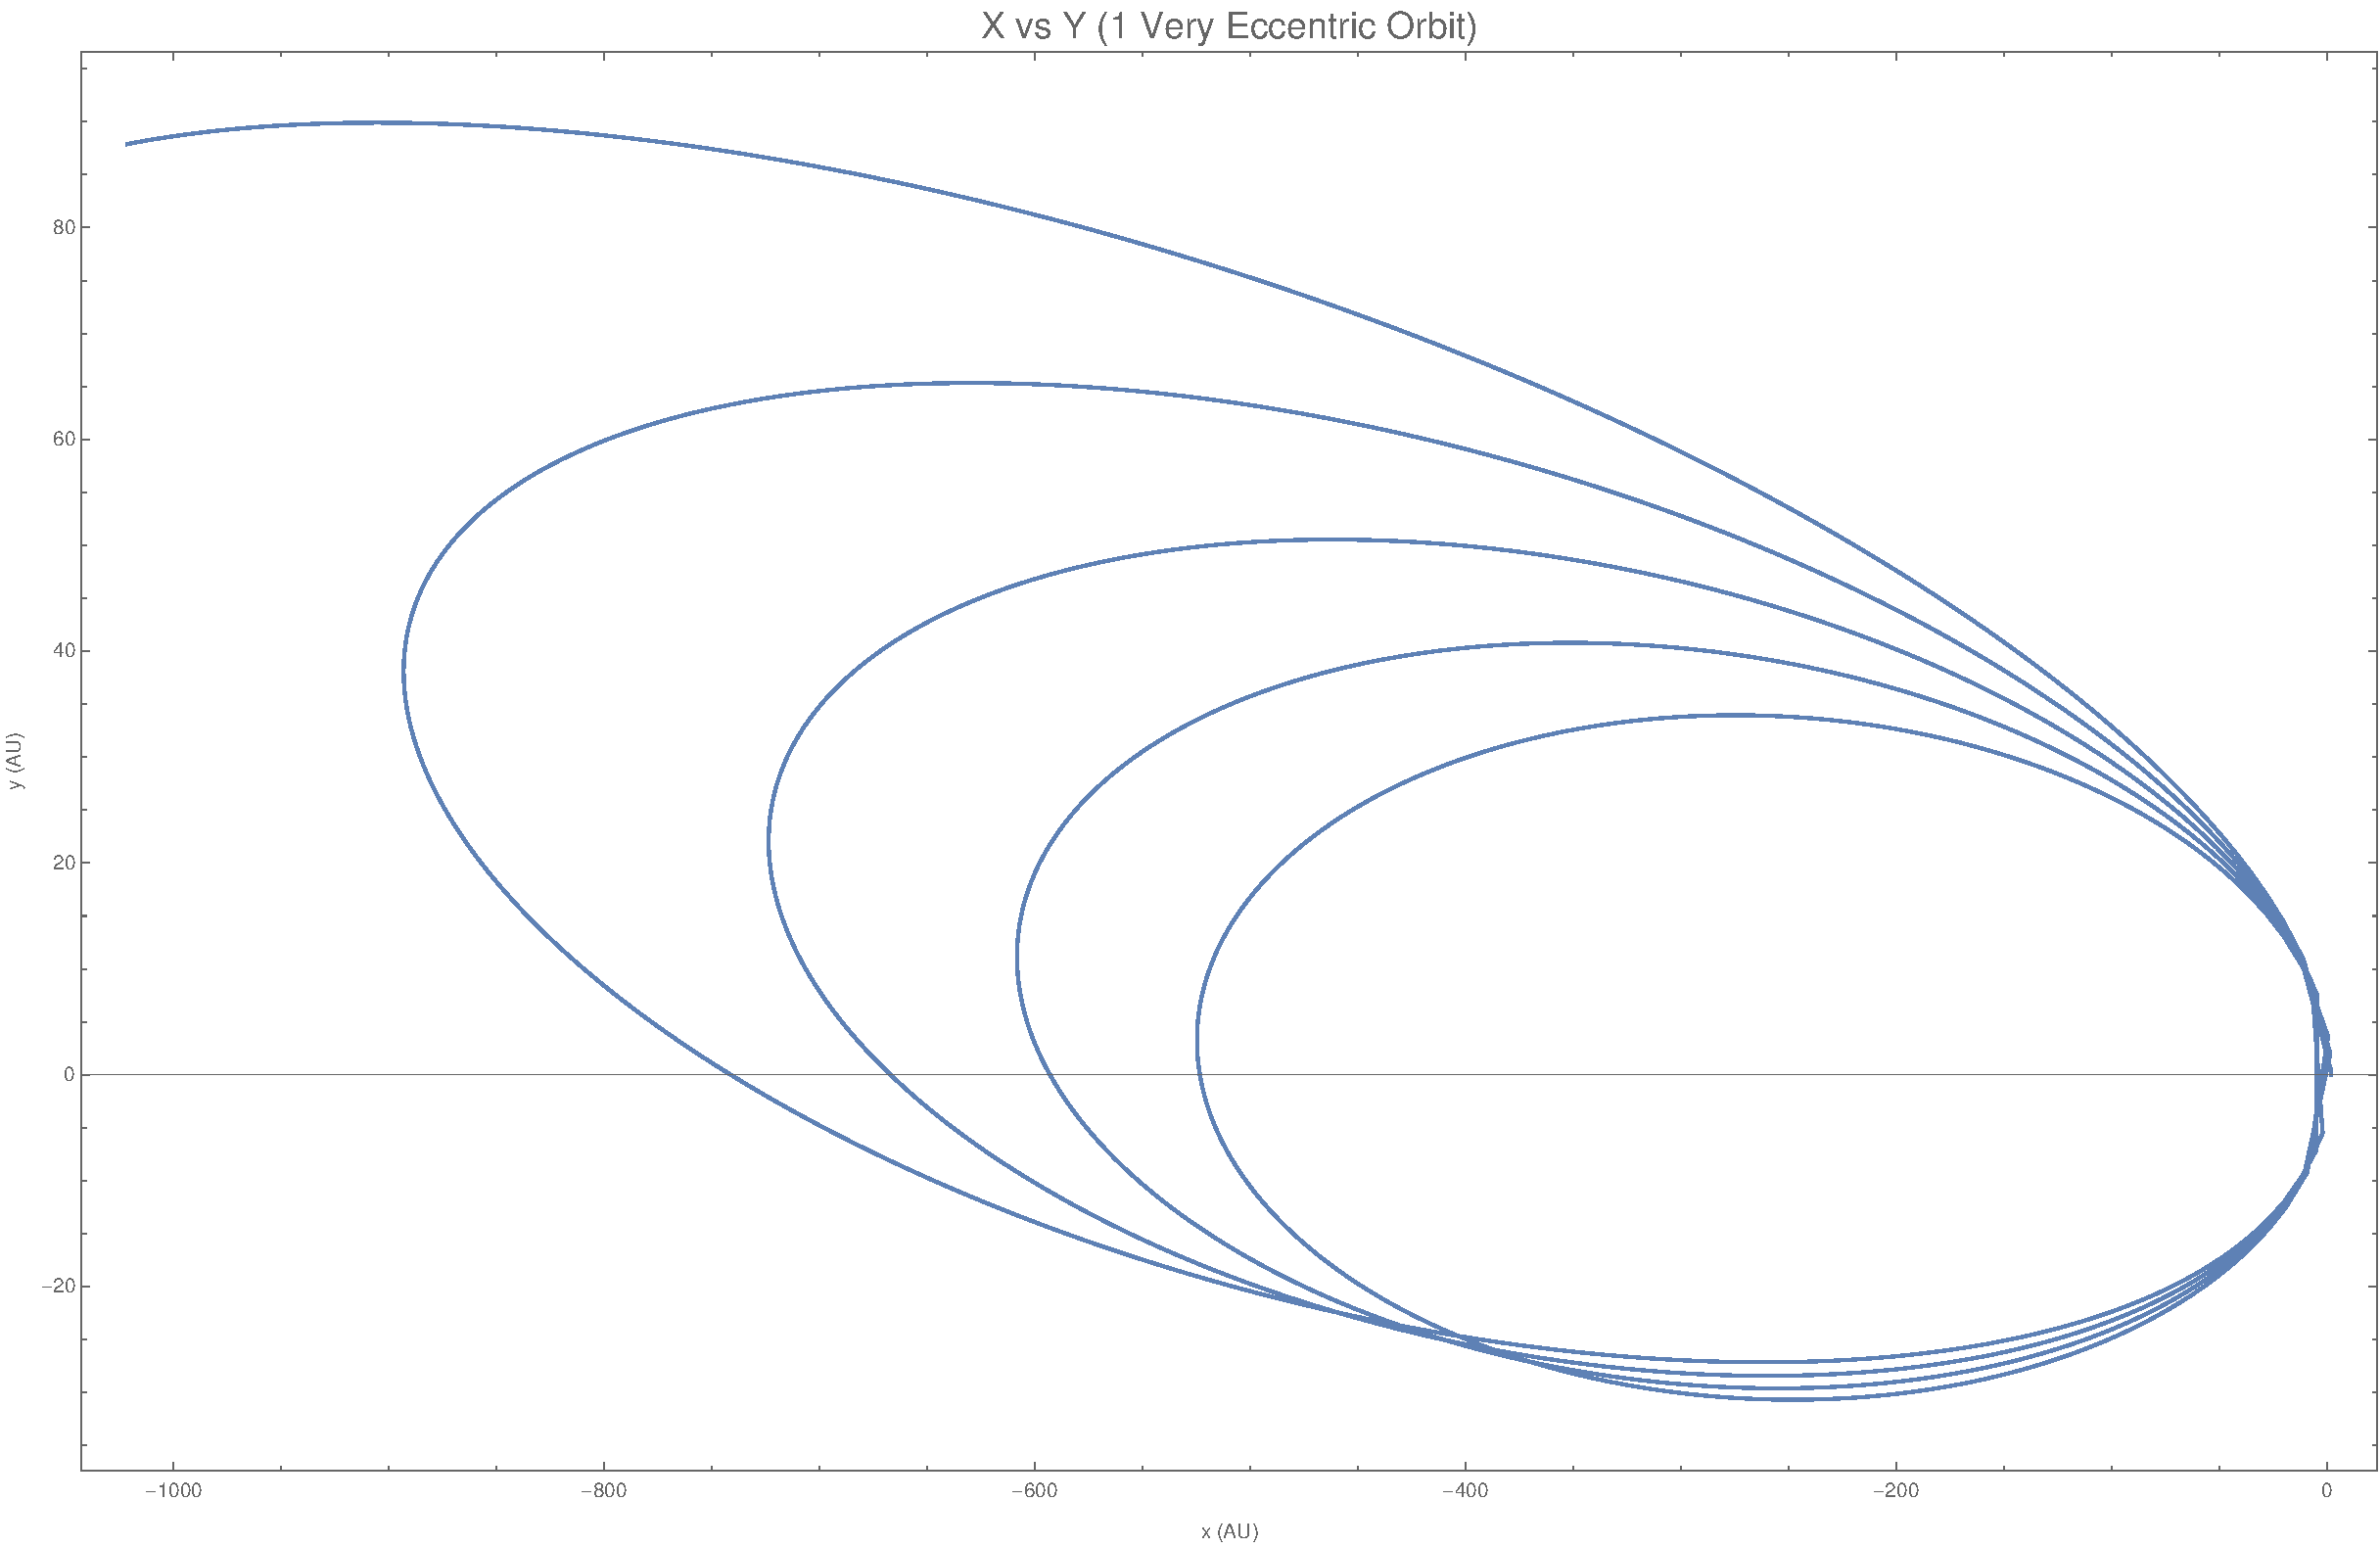
\includegraphics[width=0.4\textwidth]{veo.pdf}
	\end{center}
	\caption{Something isn't right with our simulation. The planet shouldn't be leaving, yet is seems to get slingshot out of the system.}
	\label{fig:veo}
\end{figure}

\begin{figure}[h]
	\begin{center}
		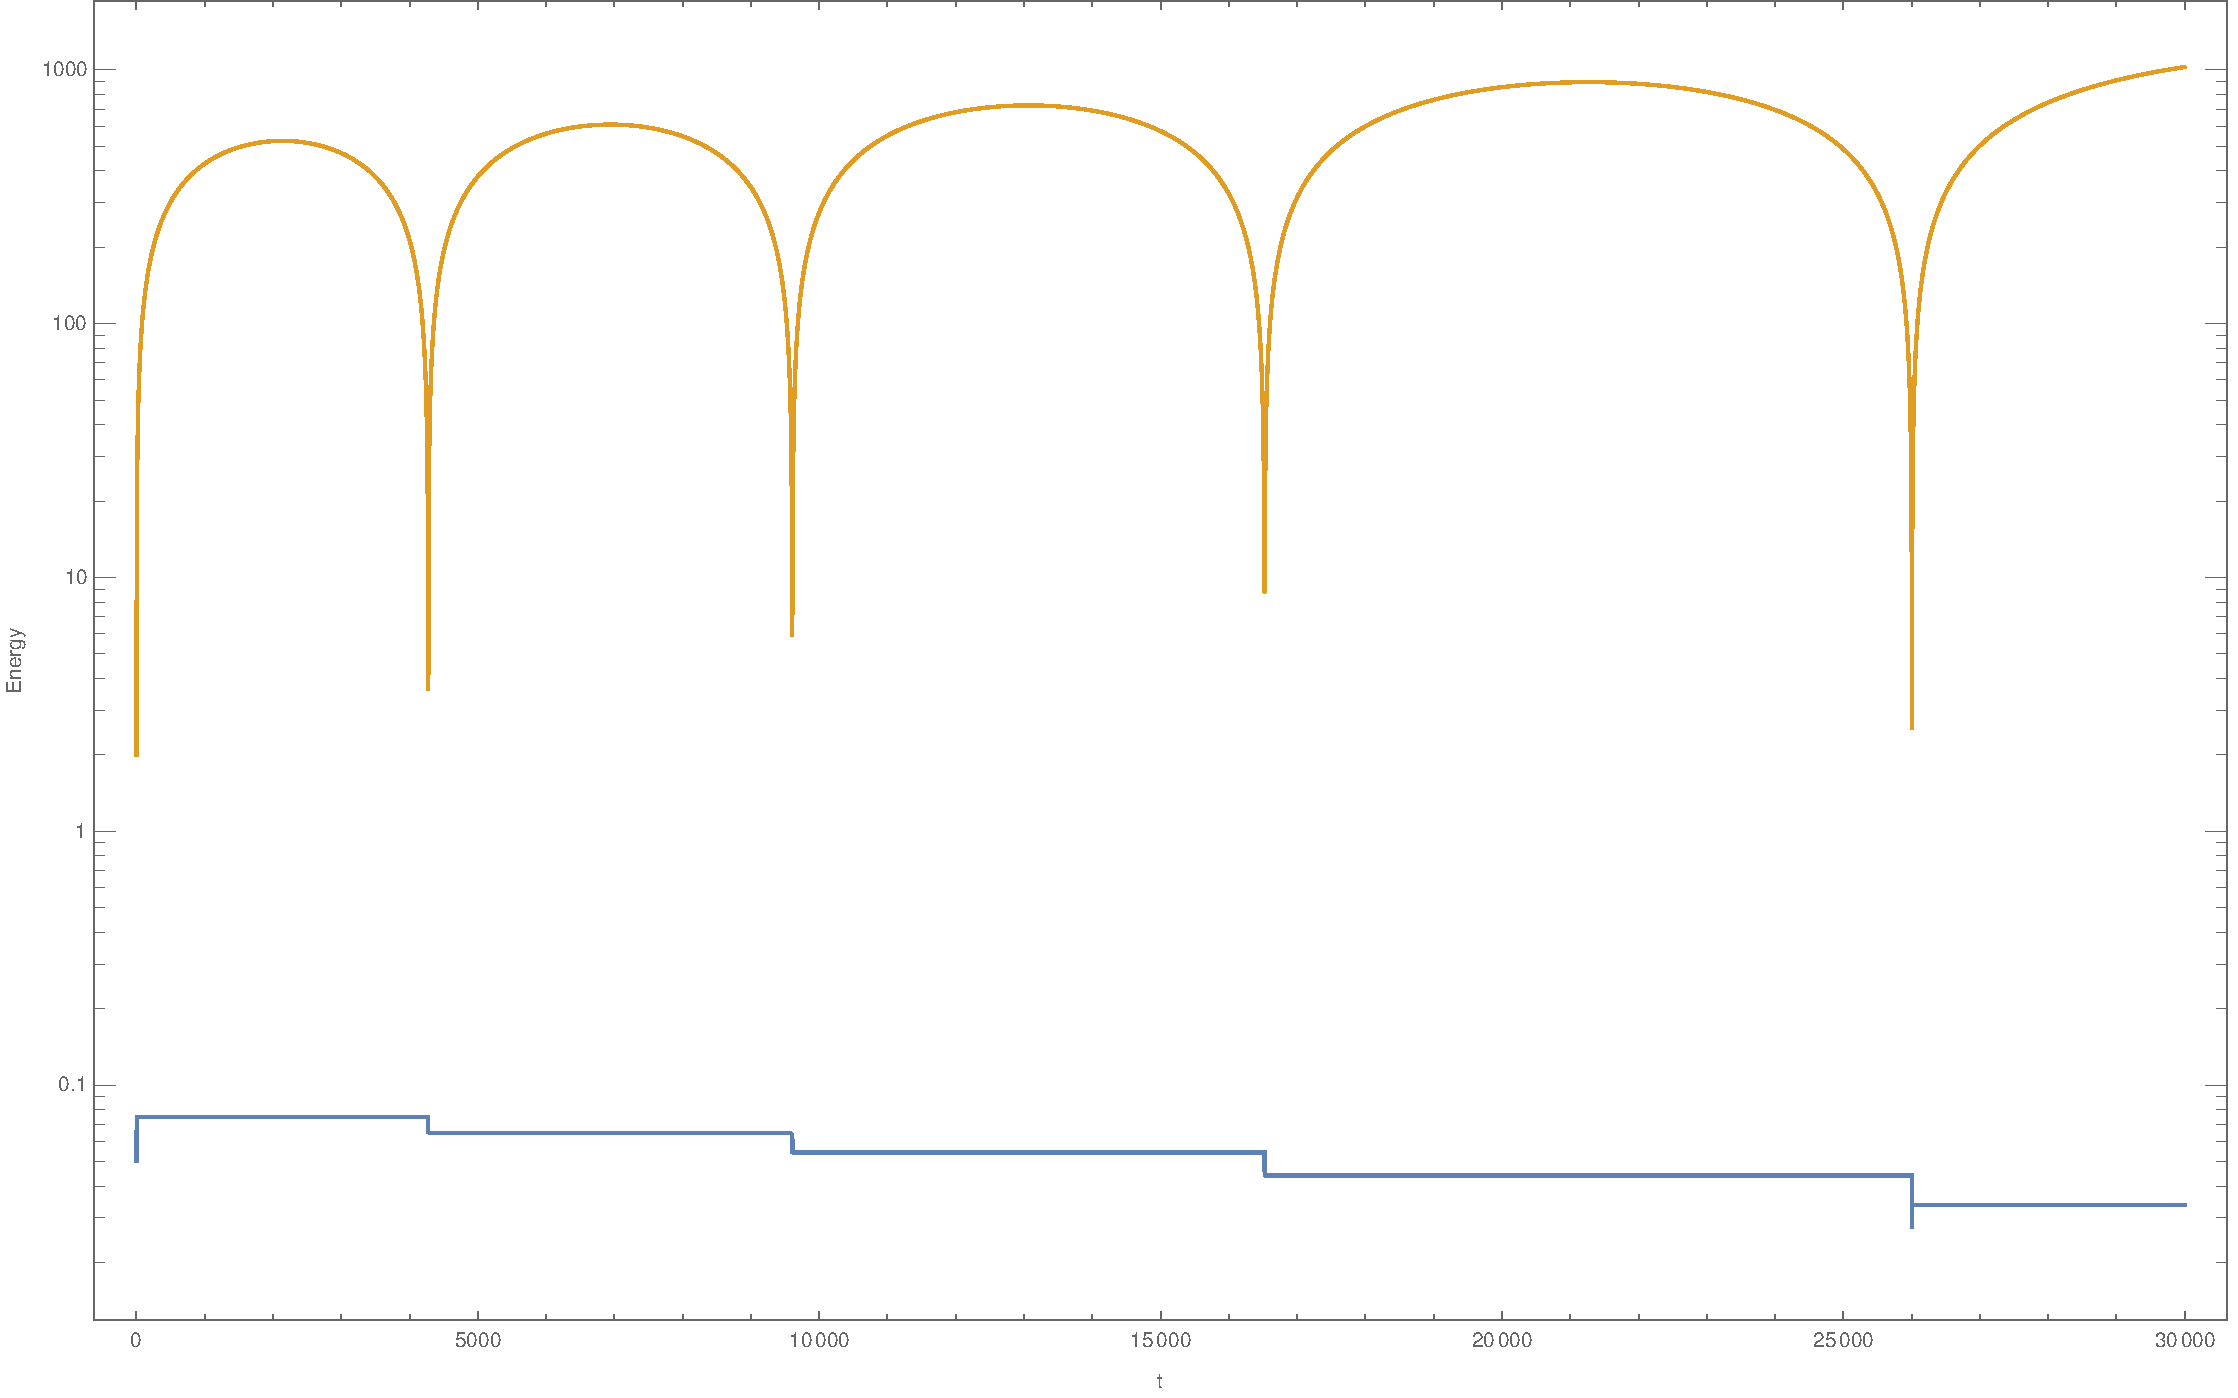
\includegraphics[width=0.4\textwidth]{ver.pdf}
	\end{center}
	\caption{In the graph above we see radius of the orbit and the absolute value of the total energy. Every time the radius gets smaller energy seems to leak into the simulation.}
	\label{fig:veo}
\end{figure}

For Highly eccentric orbits, a loss of precision of the simulation occurs every time the planet passes through the perigee. For highly elliptical orbits this happens because during the passing of perigee there is a rapid change in both the direction and velocity of the orbiting body, the RK2 algorithm is insufficient to keep up with these rapid changes and would need to use a shorter timescale to preserve accuracy. However, long orbits means that a lot of extra computation is required for this solution. Where much of the time the larger time step would be sufficient.

\pagebreak
\bigskip
\noindent{\bf Bonus}
\medskip

No, these orbits are no longer elliptical. Once we move to a universe where gravity scales with $\frac{1}{r^3}$ energy is not conserved in orbital mechanics and any small deviation from a perfectly circular orbit will lead to the planet being ejected from orbit, as we can see in Figure \ref{fig:r3}. The initial condition for this system was a radius 1 part in 10000 larger than perfectly circular. Over a 20 year period the planet is flung further and further into space.

If you look at Figure \ref{fig:r3e} we can see that the total energy of the system is not conserved.

\begin{figure}[h]
	\begin{center}
		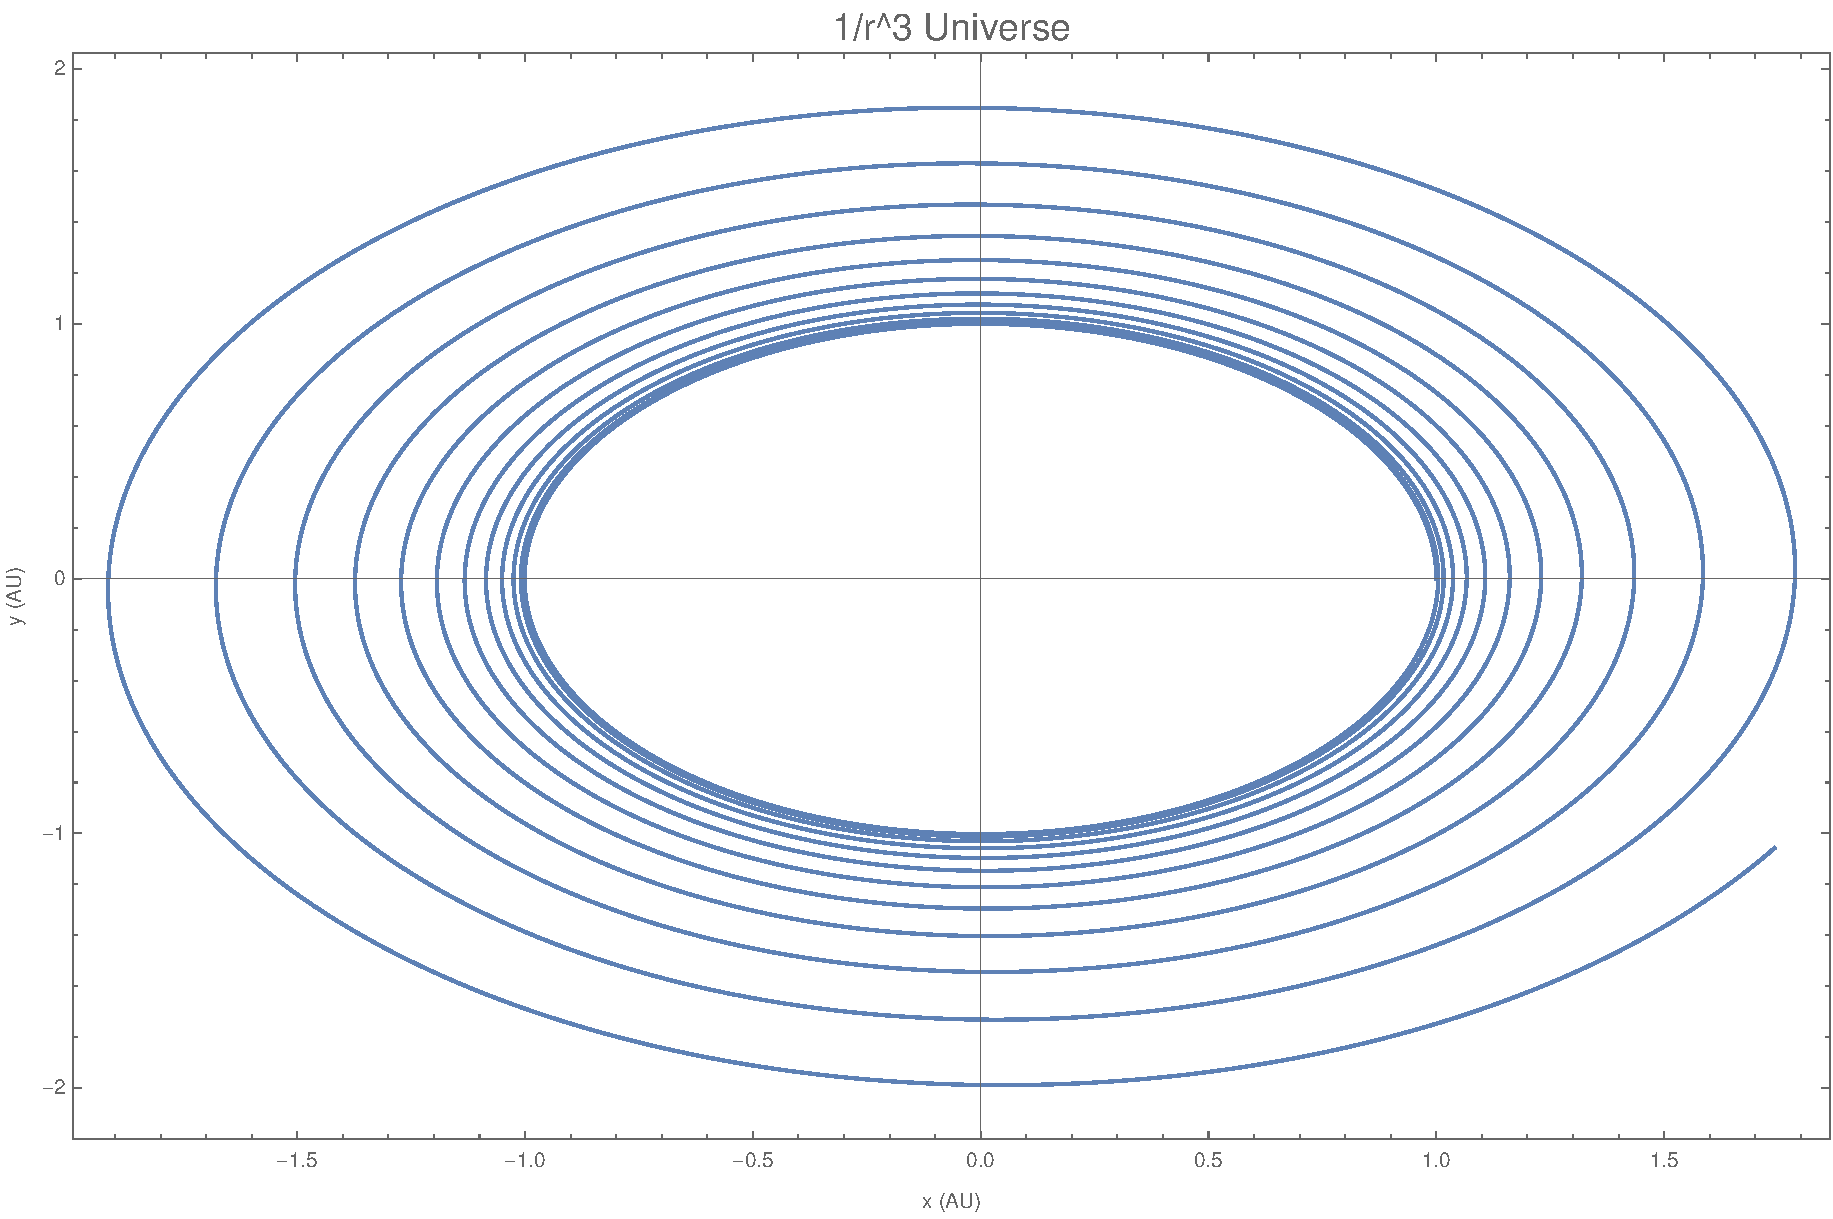
\includegraphics[width=0.4\textwidth]{r3.pdf}
	\end{center}
	\caption{The tiniest nudge can fling a planet out of orbit in this system.}
	\label{fig:r3}
\end{figure}


\begin{figure}[h]
	\begin{center}
		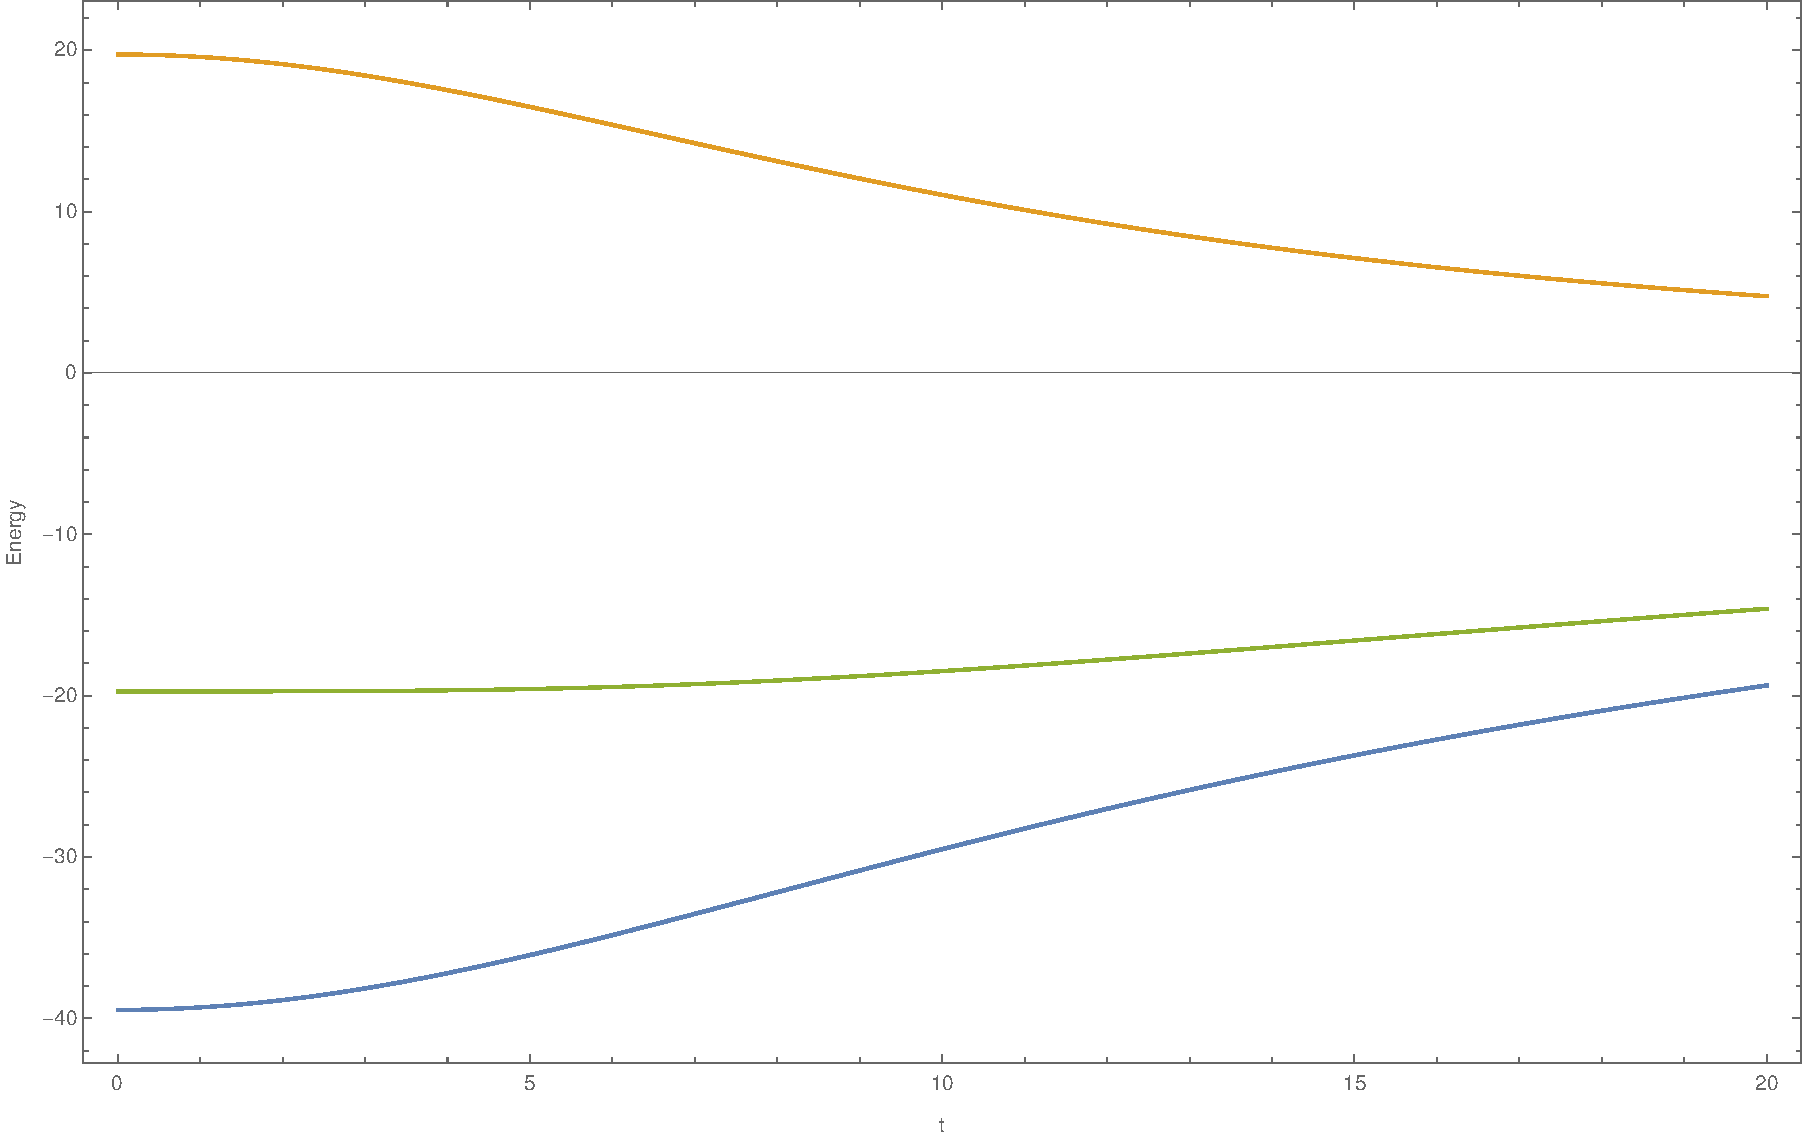
\includegraphics[width=0.4\textwidth]{r3e.pdf}
	\end{center}
	\caption{Energy is no longer conserved in this system. Energy bleeds into the system and the planet is flung out into space. Green is the Total Energy of the system, Orange is the Kinetic Energy, and Blue is the Potential Energy.}
	\label{fig:r3e}
\end{figure}

\section{Conclusions}

Rutta-Kunga method provides a much quicker method of approximating solutions to differential equations than Euler's Method. Also there is a rather nice package for vim called `xuhdev/vim-latex-live-preview' it really simplifies the process of writing \LaTeX. Additionally I managed to find the problem with Mathematica crashing on file saves. If more than one Kernel is open then they can conflict in file browser \texttt{SetDirectory}. When that happens Mathematica freezes and all progress can be lost.

\end{document}
